\section{Deterministic Model}
\label{sec:model}
We subdivide the classic SIRD compartments, Susceptible ($S$), Infectious ($I$), Recovered ($R$) and Deceased ($D$), with sub-compartments allowing for heterogeneous areas of residence and vaccination states as well as infections by different virus types. Individuals either live in area $A$ or area $B$. They are non-vaccinated $v_0$, vaccinated with vaccine one $v_1$ or vaccinated with vaccine two $v_2$. We introduce two virus types. A wild type $w$ that serves as baseline variant and a more infectious mutant $m$ variant.
\begin{figure}[h!]
\centering
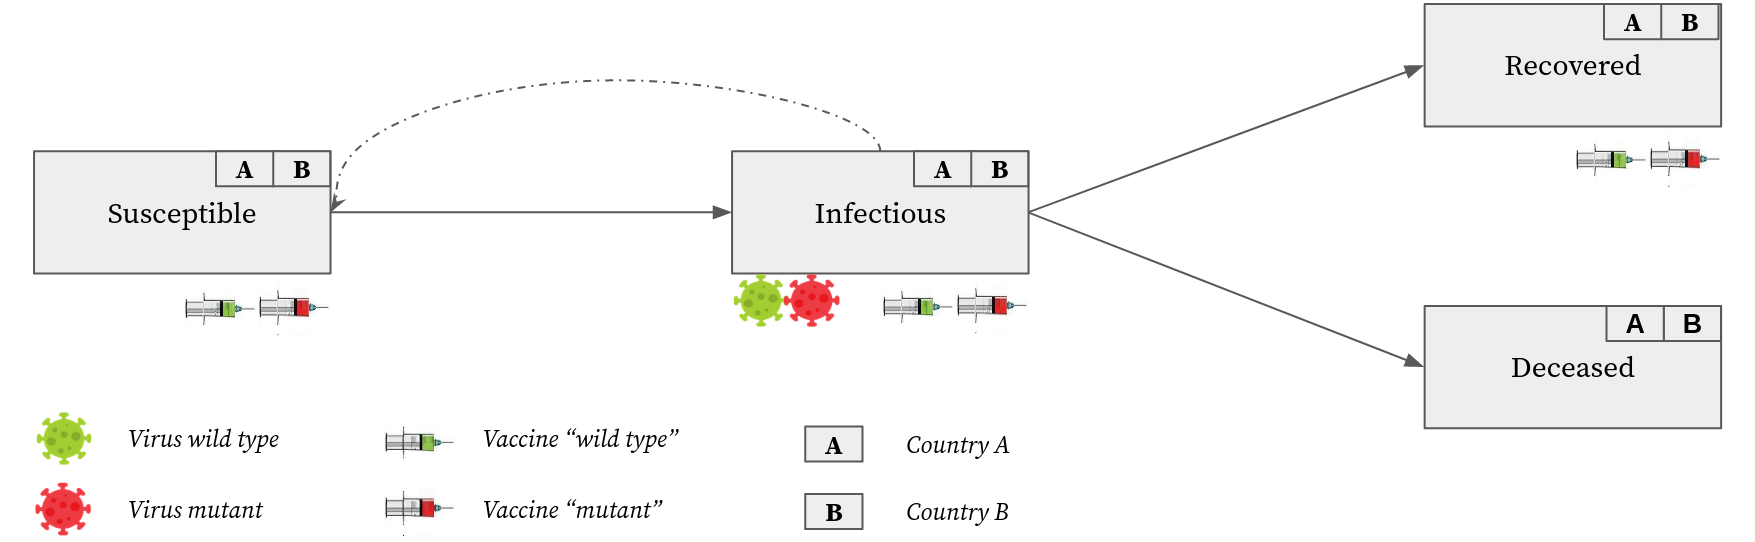
\includegraphics[scale=0.23]{images/vaccination_pp.png}
\caption{Compartments }
\end{figure}
To describe our model we follow the notation in \cite{Waites.2021} and denote every sub-group of individuals by a set $\set(F_n)$, where $F_n$ is a placeholder for features of individuals the set $\set$ is representing and $t$ denotes the time at which the set is evaluated. We illustrate this in the following by examples. Let $X_i$ for $i \in \{S, I, R, D \}$ indicate to which general compartment an individual belongs, then, $\set(X_S)$ is the set of all susceptible individuals and $\set(X_I)$ is the set of all infectious individuals in $t$. If we want to distinguish not only between general compartments but additionally between countries of residence, we use the feature $C_j$ for $j \in \{A, B\}$ to indicate that the country of residence is $j$. $\set(X_S, C_A)$ is the set of all susceptible individuals of country A and $\set(X_S, C_B)$ of country B. Note that the ordinary set operators apply, allowing us to us linkages such as $\set(X_S, C_A) \cup \set(X_S, C_B) = \set(x_S)$ or $\set(X_S) \cap \set(X_I) = \emptyset$. The negation operator $\neg$ is used to indicate that a certain feature applies for all but the specified compartment, e.g. $\set(\neg X_D)$ is the set of all alive individuals. The cardinality $|\cdot|$ represents the respective number of individuals in a set, e.g. $|\set(X_S)|$ equals the number of all susceptible individuals. To shorthand notation, we define $\num(F_n) = |\set(F_n)|$ as the number of individuals in the compartment addressed by $(F_n)$. \\ By definition $\set() = \cup_{i \in \{ S, I, R,D\}} \set(X_i)$ is the set of all individuals. An overview of all features is given in Table \ref{tab:features}. 
\begin{table}[h!]
\centering
\caption{Notation}
\label{tab:features}
\begin{center}
\scalebox{0.8}{
\begin{tabular}{lclp{10cm}}
\hline
\multicolumn{1}{l}{Feature}&\multicolumn{1}{c}{Code}&\multicolumn{1}{c}{Indices}&\multicolumn{1}{c}{Explanation}\\
\hline
\rule{0pt}{2.6ex}General compartment & $X_h$ &  $h \in \{S, I, R, D\}$ & Individuals can either be Susceptible ($S$), Infectious ($I$), Recovered ($R$) or Deceased ($D$). \\
Country of residence & $C_j$ &  $j \in \{A, B\}$ & Individuals can either live in country A or country B.  \\
Virus Type & $V_k$ &  $k \in \{W, M\}$ & An infection can either be caused by the wild type ($W$) or the mutant ($M$) virus. This feature has to be understood, depending on $X_h$, as \textit{is} or \textit{has been} infected with type $k$. For example an individual of $\set(X_I, V_k)$ \textit{is} currently infected and an individual of $\set(X_R, V_k)$ \textit{has been} infected.\\
Vaccine Type & $U_l$ &  $l \in \{0, 1, 2\}$ & An individual can either be vaccinated with vaccine 1 or 2 or being unvaccinated ($U_0$). \\
Placeholder & $F_i$ &  $i \in \mathbb{N}$ & A placeholder that is used to address an arbitrary combination of features. $\set(F_i)$ should be read as the set of a fixed but arbitrary compartment. If we need to distinguish between two arbitrary compartments, we use $F_1$ and $F_2$.\\
\hline
\end{tabular}
}
\end{center}
%\begin{tablenotes}
%\scriptsize
%\item Note: 
%\end{tablenotes}
\end{table}

We do not incorporate reinfections. Thus, a susceptible individual cannot be associated with any virus type and therefore $\set(X_S, V_k) = \emptyset$ for all $k \in {W,M}$. Moreover, we impose a set of assumptions to our model. 
\begin{assumption}\label{ass:model}
For all $t,r \in \R_+$ and $s \in [-t, \infty)$ let
\begin{align*}
\tag{\ref{ass:model}.1} 
\label{eq:no_reinfections}
\set(X_I, V_k) \cap \mathcal{C}_{t+r}(X_S) &= \emptyset \\
\tag{\ref{ass:model}.2} 
\label{eq:no_double_vaccinations}
\set(U_1) \cap \mathcal{C}_{t+s}(U_2) &= \emptyset \\
\tag{\ref{ass:model}.3} 
\label{eq:no_cross_border_mobility}
\set(C_A) \cap \mathcal{C}_{t+s}(C_B) &= \emptyset 
\end{align*}
\end{assumption}
Assumption \ref{eq:no_reinfections} rules out reinfections. An individual that has been infected once cannot become reinfected after it had recovered. According to recent studies \textbf{cite paper} this is not true for COVID-19. However, the number of reinfected individuals is negligible and we therefore do not incorporate reinfections to keep our model parsimonious. Assumption \ref{eq:no_double_vaccinations} implies that an individual only receives one type of vaccine. Receiving one vaccination shot in our model implies that an individual is fully protected according to the vaccine properties making it unrealistic to assign a second shot to this individual. Assumption \ref{eq:no_cross_border_mobility} rules out permanent cross-country movements of individuals. According to \textbf{cite how many individuals move from one to another country} the number is negligible. We therefore decided to leave out permanent changes of residence. However, we incorporate cross-border infections via meeting rates within the mass actions.

\subsection{System of ordinary differential equations}
Since we use a compartment SIRD model based on a system of ordinary differential equations (ODEs) and to make this thesis self-contained, we review how the dynamics of a chemical reaction network are modeled over time. We can limit ourselves to the case of irreversible reactions since recovered and deceased individuals cannot become infectious again and infectious individuals become recovered but not susceptible. Let $\set(F_1), \dots, \set(F_n)$ be $n$ disjoint sets. Every irreversible reaction $R_j$, for $j = 1, \dots, m$, can be expressed as
\begin{align}
\nu_{1j} \num(F_1) + \hdots + \nu_{nj} \num(F_n) \longrightarrow \mu_{1j} \num(F_1) + \hdots + \mu_{nj} \num(F_n),
\end{align}
where $\nu_{ij} \in \mathbb{N}_0$ and $\mu_{ij} \in \mathbb{N}_0$ are called stoichiometric coefficients. They describe how much of species $\set(F_i)$ is consumed $\nu_{ij}$ and produced $\mu_{ij}$ within reaction $R_j$. T difference $\mu_{ij} - \nu_{ij}$ is the total change of $\num(F_i)$ due to one reaction $R_j$. In terms of our model we are not only interested in how one reaction (e.g. an infection, a vaccination, etc.) influences the state of the system but rather how often this happens within an interval $[t, t+\tau]$, for $\tau \in \R_+$. For $\tau = 1$ the latter is described according to the law of mass action by
\begin{align}
\label{eq:change_one_unit}
v_j = r_j  \prod_{i=1}^n \num(F_i)^{\mu_{ij}},
\end{align}
where $r_j$ is a reaction specific constant. The product is the number of combinations to assign individuals from different compartments, that have $\mu_{ij} \neq 0$, together.
The change in the magnitude of $\num(F_i)$, taking into account all $m$ reactions, is given by
\begin{align}
\label{eq:sys_change}
y_{t+\tau}(F_i) - \num(F_i) = \sum_{j=1}^m (\mu_{ij} - \nu_{ij}) v_j \tau.
\end{align}
$(\mu_{ij} - \nu_{ij})$ is, as outlined above, the stoichiometry that specifies how one reaction influences the system, $v_j \tau$ is the number of times reaction $R_j$ happens within the interval $[t, t+\tau]$, and therefore the product is the influence of $R_j$ on $\num(F_i)$ during this interval. Summed over all reactions yields the change of $\num(F_i)$ in the system. We divide both sides of \eqref{eq:sys_change} by $\tau$, let $\tau \to 0$ and plug in \eqref{eq:change_one_unit} to obtain the ordinary differential equation (ODE)
\begin{align}
\der(F_i) = \sum_{j=1}^m \left[(\mu_{ij} - \nu_{ij}) r_j  \prod_{i=1}^n \num(F_i)^{\mu_{ij}} \right].
\end{align}
We write down the equations for all compartments in matrix form, determining a system of ODEs, which we will use in subsequent chapters.
\begin{align}
\label{eq:ode_system_matrix}
\underbrace{\begin{pmatrix}
\der(F_1) \\ \vdots \\ \der(F_n) \end{pmatrix}}_{Y(t)} =
\underbrace{\begin{pmatrix}
\mu_{11} - \nu_{11} & \hdots & \mu_{1m} - \nu_{1m} \\
\vdots & \vdots & \vdots \\
\mu_{n1} - \nu_{n1} & \hdots & \mu_{nm} - \nu_{nm} \\
\end{pmatrix}}_{\vect{S}} \cdot
\underbrace{\begin{pmatrix}
v_1 \\ \vdots \\ v_m
\end{pmatrix}}_{v}
\end{align}
Note that \eqref{eq:ode_system_matrix} is a linear mapping $v$ for which we can compute the kernel $\mathcal{K}=\left\{v \in \R^m | \vect{S} \cdot v = 0 \in \R^n  \right\}$. Each element of the kernel represents a state where $Y(t)=0$ and therefore the system is in a steady- state. If the pandemic reaches a state such that $v \in \mathcal{K}$, we would be stuck there. \textbf{write how the null space looks like in our model} \\

Since our model consists of over 100 reactions, we do not write down the ODE system explicitly. However, it can be constructed as stated in this section.  
\subsection{Reactions}
We divide the reactions in three groups: Infections, Recoveries and Deaths, Vaccinations. We group recoveries and deaths together, since they have the same structure. To define a reaction, we must specify the reactants, products, their stoichiometric coefficients and the reaction constants. For each reaction group we first state the general reactions, defining the reactants, products and stoichiometric coefficients, build intuition for it, subsequently specify the reaction constant, and state the reactions explicitly.


\subsubsection{Infections}
Every infection happens between an infectious individual $i_1 \in \set(x_I)$ and a susceptible individual $i_2 \in \set(x_S)$ and leads to two infectious individuals. Hence, the general form of the infection reactions is
\begin{align}
\label{eq:general_infection}
\num(x_I, F_1) + \num(x_S, F_2) \longrightarrow \num(X_I, F_1) + \num(X_I, F_2),
\end{align}
where we use $F_1, F_2$ to indicate that the reactions differ with respect to not explicitly mentioned features, e.g. vaccinated individuals have a lower risk of becoming infected or transmitting the virus, the mutant virus is more infectious, and cross-border infections are scaled by a factor to make them comparatively rare events. %If $F_1 \neq F_2$, the stoichiometric coefficients are one and if $F_1=F_2$, they are one for the reactants and two for the products. 
The additional features represented by $F_1$ and $F_2$ are incorporated within the reaction constants
\begin{align*}
\text{infection constant} = \text{contacts} \times \text{infectiousness} \times \text{vaccine modifier} 
\end{align*}
In the following we elaborate on how to define each component of the infection constants.\\

\textbf{Infectiousness.} Let $c \in R_+$ be the average number of contacts per individual and day and $\alpha \in [0,1]$ be the proportion of susceptible individuals that become infected if they meet a wild type infected individual without any vaccination of both individuals. Let $\eta \in (1, 1/\alpha]$ be the factor with which the mutant is more infectious than the wild type. Then $\beta = \alpha c$ is the average number of individuals infected per day by $i_1$ if $i_1 \in \set(X_I, V_w, U_0)$. If $i_1 \in \set(X_I, V_M, U_0)$ the average infected number increases to $\eta \beta$. \\

\textbf{Vaccine modifier.}
To account for the influence of vaccines on vaccinated susceptible individuals, we introduce the parameters $\delta_{k,l} \in [0,1]$, where $k \in \{W, M\}$ indicates the virus type and $l \in \{ 1,2\}$ the vaccine type. If $i_2 \in \set(X_S, U_l) $ for all individuals that $i_1 \in \set(X_I, V_k)$ meets, the infection rate is multiplied by $1 - \delta_{k,l}$, and thus the reaction constant in the respective reaction. Hence, $\delta_{k,l}$ is interpreted as reduce in the probability of becoming infected while meeting an infectious individual.

Moreover, vaccinated individuals have a lower probability of transmitting the virus (\textbf{Quelle}). We account for this by introducing the parameter $\gamma \in [0,1]$ and multiplying the average number of infected individuals by $(1 - \gamma)$ if $i_1 \in \set(X_I, U_1) \cup \set(X_I, U_2)$. $\gamma$ is the reduction in the probability of not transmitting the virus after being vaccinated. We assume that $\gamma$ is constant over time and across vaccines (\textbf{Quelle}). \\

\textbf{Contacts.}
We want to distinguish between how many of the average contacts per day $c$ are within individuals from the same country and how many are within individuals from another country. We do so by defining probabilities that given a meeting occurs, it is with an individual from another country and multiply $c$ with the respective probability to obtain the average number individuals infected by one individual in a certain country. We use the relative population number of a country as baseline probability and add a penalty term for cross-border meetings. 

In the following we establish how we specify all probabilities. We first define the (time dependent) probability that a randomly drawn living individual $i_2$ lives in country $B$ 
\begin{align}
\prob_t\left(i_2 \in \set(\neg X_D, C_B)\right) =\num(\neg X_D, C_B) / \num(\neg x_D).
\end{align}
The probability depends on the state of the whole system $Y(t)$. To increase readability we omit conditioning on $Y(t)$ and directly define $\prob_t$ to be conditioned on the state of the system $Y(t)$.  
Second, we define the conditional probability that given $i_1$ is from country A, $i_2$ is from country B by adding a multiplicative penalty term $b(\cdot)$ reducing the probability of meeting individuals from other countries 
\begin{align*}
\prob_t(i_2 \in \set(\neg X_D, C_B) | i_1 \in \set(\neg X_D, C_A) ) = \prob_t\left(i_2 \in \set(\neg X_D, C_B)\right) \cdot b(d(A, B)),
\end{align*}
where $d(A, B)$ is a distance between country $A$ and country $B$ and $b: \R_+ \to [0,1]$  is a function that maps the distance to the penalty value. By mapping the distance into the unit interval, we allow the probability of a cross-border meeting to be maximally as high as the relative population size. The distance can be interpreted as geographical distance. However, it could also serve to incorporate other factors, like favored holiday destinations, that encourage or discourage cross-border meetings. We impose three conditions on the function $b$
\begin{align}
\lim_{b \to \infty} &= 0 \tag{B.1}\\
b(0) &= 1 \tag{B.2}\\
b(d_1) &< b(d_2) \quad \textrm{if } d_1 > d_2. \tag{B.3}
\end{align}
Condition $(B.1)$ ensures that countries that a very large distance only have small influences onto each other, $(B.2)$ defines a rather theoretical case where cross-border meetings are as likely as within-country meetings, and $(B.3)$ ensures that countries that have a greater distance have a smaller influence on each other. We define all possible conditional meeting probabilities depending on the countries of residence analogously. To increase readability when we define the reaction rates explicitly below, we collect them in a matrix $\vect{M} \in \R^{2 \times 2}$, such that we can address them via $m_{j_1,j_2}$ for $j_1, j_2 \in \{A, B\}$
\begin{align}
\label{eq:matrix_M}
\vect{M} &= \begin{pmatrix} 
m_{A,A} & m_{A,B} \\
m_{B,A} & m_{B,B} 
\end{pmatrix} \\
&= \begin{pmatrix} 
\prob(i_1 \in \set(\neg X_D, C_A) | i_1 \in \set(\neg X_D, C_A) ) & \prob(i_1 \in \set(\neg X_D, C_A) | i_2 \in \set(\neg X_D, C_B) ) \\
\prob(i_2 \in \set(\neg X_D, C_B) | i_1 \in \set(\neg X_D, C_A) ) & \prob(i_2 \in \set(\neg X_D, C_B) | i_2 \in \set(\neg X_D, C_B) )
\end{pmatrix} \notag \\
&= \begin{pmatrix} 
1 - \num(\neg X_D, C_B) / \num(\neg X_D)   & \num(\neg X_D, C_A) / \num(\neg X_D)  \\
\num(\neg X_D, C_B) / \num(\neg X_D)  & 1 - \num(\neg X_D, c_A) / \num(\neg X_D)
\end{pmatrix} \cdot b\left(\text{d}(a_1, a_2) \right). \notag
\end{align} 

%The negation operator $\neg$ is used to indicate that a certain feature applies for all but the specified compartment, e.g. $\set(\neg x_D)$ is the set of all alive individuals. We specify the probability of an individual $i_1 \in \set()$ to be in a particular subset by its relative frequency. For example, the (time dependent) probability that a randomly drawn living individual $i_1$ lives in country $A$ is $\prob_t\left(i_1 \in \set(\neg x_I, c_A)\right) =\num(\neg x_D, c_A) / \num(\neg x_D)$. Analogously, we can compute the probability the individual is from country A and susceptible by $\prob_t\left(i_1 \in \set(x_S, c_A)\right) = \num(x_S, c_A)/\num(\neg x_D)$. To compute the probability that the individual is susceptible, conditioned that it is from country $A$, we can use Bayes' formula 
%\begin{align}
%\prob_t\left( i_1 \in \set(x_S) |  i_1 \in \set(\neg x_D, c_A) \right)= \frac{\prob_t\left(i_1 \in  \set(x_S, c_A) \right)}{\prob_t\left(i_1 \in \set(\neg x_D, c_A)\right)} = \frac{\num(x_S, c_A)}{\num(\neg x_D, c_A)},
%\end{align}
%which yields just the proportion of susceptible individuals in country A.\\

Since we are interested in specifying an infection reaction for each compartment, we show subsequent how we define the average numebr of contacts for concrete $F_1$ and $F_2$ from \eqref{eq:general_infection}. We set $i_2 \in \set(X_S, C_B, U_0)$ and $i_1 \in \set(X_I, V_W, C_A, U_0)$. We need conditional probability $\prob_t(i_2 \in \set(X_S, X_B, U_0)|i_1 \in \set(X_I, V_W, C_A, u_0))$. This to say, the probability that the individual that can be infected ($i_2$) is susceptible, unvaccinated and from area two given that individual $i_1$ is infected with the wild type, unvaccinated and from area one. We facilitate our model and assume that the vaccination status as well as the type of virus infection of individual $i_1$ are independent of the features of $i_2$. Assuming independence of the vaccination status implies that an unvaccinated individual $i_1$ does not change her contact habits, given a certain number of meetings, compared to her counterfactual vaccinated self. Note that this does not mean that we assume that vaccinated and unvaccinated individuals have the same average number of contacts since the probabilities are defined on \textit{conditioned a meeting occurs}. Differences in the average number of contacts between vaccinated and unvaccinated individuals can be incorporated implicitly via the vaccination parameter $\delta_{k,l}$. 

Furthermore, we assume that the probability is dependend on whether an individual is alive but not on the exact general compartment $S, I$ or $R$. Making use these assumptions, we can omit conditioning on $V_w$ and $U_0$ and change $X_I$ to $\neg X_D$ such that the exercise facilitates to defining $\prob_t(i_2 \in \set(X_S, C_B, U_0)|i_1 \in \set(\neg X_D, C_A))$. Using Bayes' formula we can rewrite this as
\begin{align}
\label{eq:cond_meeting_prob}
\prob_t(i_2 \in \set(X_S, C_B, U_0)|i_1 \in \set(\neg X_D, C_A)) &= \prob_t(i_2 \in \set(\neg X_D, C_B) | i_1 \in \set(\neg X_D, C_A) )  \notag \\
& \quad \cdot \prob_t(i_2 \in \set(X_S, U_0) | i_1 \in \set(\neg X_D, C_A), i_2 \in \set(\neg X_D, C_B) ) \notag \\
&= \prob_t(i_2 \in \set(\neg X_D, C_B) | i_1 \in \set(\neg X_D, C_A) )  \notag \\
& \quad \cdot \prob_t(i_2 \in \set(X_S, V_0)|i_2 \in \set(\neg X_D, C_B)) \notag\\
&= \prob_t(i_2 \in \set(\neg X_D, C_B) | i_1 \in \set(\neg X_D, C_A) ) \notag \\
& \quad \cdot \prob_t(i_2 \in \set(X_S, C_B, V_0))
\end{align} 
The conditional probability is therefore the product of the probability that $i_2$ is from country $B$ given that $i_1$ is from country $A$ and the probability that $i_2$ is a susceptible, unvaccinated individual from country $B$. Using equations \eqref{eq:matrix_M} and \eqref{eq:cond_meeting_prob} we obtain
\begin{align}
\label{eq:cond_prob_meeting_final}
\prob_t(i_2 \in \set(X_S, C_B, U_0)|i_1 \in \set(X_I, V_W, C_A, U_0)) = m_{B,A} \cdot \num(X_S, C_B, U_0) / \num(\neg X_D, C_B). 
\end{align}


\textbf{Explicit reactions.}
With the derived probabilities we are able to specify the compartment specific infection constants. We illustrate this by two examples. 

The first example deals with the compartments $\set(X_{I}, C_A, V_W, U_0)$ and $\set(X_{S}, C_B, U_0)$. The corresponding reaction is
\begin{align}
\num(X_{I}, C_A, V_W, U_0) + \num(X_{S}, C_B, U_0) &\xrightarrow{ r_{j_1}} \num(X_{I}, C_A, V_W, U_0) + \num(X_{I}, C_B, V_W, U_0),
\end{align}
where $r_j$ denotes the reaction rate.
By assumption, every individual $i_1 \in \set(X_{I}, C_A, V_W, U_0)$ has on average $c$ contacts per day. Equation \eqref{eq:cond_prob_meeting_final} defines the fraction of contacts which are between the two compartments of interest. Since both compartments are non-vaccinated compartments and $i_1 \in \set(V_W)$ the fraction of infectious contacts is $\alpha$. Thus, $i_1$ infects on average $\beta m_{B,A} \cdot \num(X_S, C_B, V_0) / \num(\neg X_D, C_B)$ susceptible, unvaccinated individuals from country B. Both individuals are non-vaccinated and therefore the vaccine modifier is simply one. The respective infection constant is given by
\begin{align}
r_{j_1} = \frac{\beta \cdot m_{B,A} }{ \num(\neg X_D, C_B) } 
\end{align}
For the second example, we consider vaccinated and mutant infected compartments $\set(X_{I}, C_A, V_M, U_1)$ and $\set(X_{S}, C_B, U_2)$ to showcase the influence of the vaccine and the mutant modifier. 
\begin{align}
\num(X_{I}, C_A, V_M, U_1) + \num(X_{S}, C_B, U_2) &\xrightarrow{ r_{j_2}} \num(X_{I}, C_A, V_M, U_1) + \num(X_{I}, C_B, V_M, U_2).
\end{align}

We derive the infection constant analogously to the previous example. Using the vaccine modifiers $\gamma$, $\delta_{M, 2}$ and the increase in infectiousness of the mutant $\eta$ 
\begin{align}
r_{j_2} = \frac{(1-\delta_{M,2}) (1-\gamma) \eta \beta \cdot m_{B,A} }{ \num(\neg x_D, c_B) }.
\end{align}
Technically we multiply $\alpha$ by $(1-\delta_{M,2}) (1-\gamma)$ to reduce the degree of infectiousness accounting for vaccinations and increase it by multiplying it by $\eta$, to account for the more infectious mutant. 
To ensure readability we refrain from writing down all exact infection rules. They are defined for all possible combinations of features $F_1$ and $F_2$. Their infection constants can be derived analogously to what we have showcased.

\subsubsection{Infectious to Recovered/Deceased}
The transition from the infectious state to the recovered or deceased state is independent of any other compartments. The general reactions are
\begin{align}
\label{eq:recovery}
    \set(X_I, F_1) & \longrightarrow  \set(X_D, F_1) \\
    \set(X_I, F_2) & \longrightarrow  \set(X_R, F_2). \notag
\end{align}
Defining the reaction constants, depends on the state of the product, deceased or recovered and on the vaccination status, since vaccinated individuals have a much lower probability of having severe course of disease \textbf{Quelle}. 

For $\lambda \in \R_+$ we assume that on average an individual stays $1/\lambda$ days in the infectious state before it transmits either to the recovered or the deceased state. Thus, on average $\lambda$ individuals transmit out of each infectious compartment every day. We assume that a fraction $p \in [0,1]$ of unvaccinated individuals transmits to the deceased state and $(1-p)$ to the recovered state. Note that the assumption that deceasing and recovering individuals might not hold in reality, since recovering individuals might not be infectious as long as deceasing individuals. However, incorporating this would raise the need for more compartments. Since we allow for vaccination of recovered and infectious individuals, this should not influence the vaccinationr ate anyways. We therefore we assume that the influence on our model results are negligible.
 
$p$ can be interpreted as the probability of dying after becoming infected. Note that $p$ does not depend on the virus type. The virus type therefore only influences the number of infections but not the probability of dying for infected individuals. \textbf{realistisch? Quelle} The explicit reactions for unvaccinated individuals are for $i \in \{A, B\}$ and $k \in \{W, M\}$
\begin{align}
    \set(X_I, C_j, V_W, U_0) &\xrightarrow{p \lambda} \set(X_D,C_j, V_w, U_0)  \\
    \set(X_I, C_j, V_w, U_0) &\xrightarrow{(1-p) \lambda} \set(X_R,C_j, V_w, U_0) \notag
\end{align}

We introduce the parameters $\omega_{k,l} \in [0,1]$, for $k \in \{W, M\}$ and $l \in \{1,2\}$, to account for the reduce in the probability of dying after being vaccinated. We use $p \omega_{k,l}$ as new probability of dying due to being infected with virus $k$ after being vaccinated with vaccine $l$.$\omega_{k,l}$ is thus the reduction in the probability of dying. The corresponding reactions for vaccinated individuals are for $i \in \{A, B\}, k \in \{W, M\}$ and $l \in \{1,2\}$
\begin{align}
    \set(X_I, C_j, V_k, U_l) &\xrightarrow{p \omega_{k,l} \lambda} \set(X_D,C_j, V_k, U_l) \\
    \set(X_I, C_j, V_k, U_l) &\xrightarrow{(1-p \omega_{k,l}) \lambda} \set(X_R,C_j, V_k, U_l) \notag
\end{align}

\subsubsection{Vaccination}
The general setting of vaccination reactions is the same as for recoveries and deaths in \eqref{eq:recovery}. Besides susceptible individuals, we allow for vaccinations of infectious and recovered individuals as well. We do the former to account for vaccinations of asymptomatic individuals (\textbf{cite 30\%}) and the latter to account for vaccination shots that are assigned to recovered individuals. \textbf{cite why recovered are vaccinated}. Let $\phi_{t, l,j} \in \R_+$ be the vaccination constant of vaccine $l$ in country $j$ at time $t$. The vaccination constant of one vaccine is assumed to be equal for all vaccination subcompartments of $S, I,R$ within one country, which is to say, that the decision of vaccinating an individual is independent whether it is susceptible, infectious or recovered.  The corresponding reactions are $j \in \{A,B\}$, $k \in \{W,M\}$ and $l \in \{1,2\}$
\begin{align}
\set(X_S, C_j, U_0) &\xrightarrow{\phi_{t,l, j}} \set(X_S, C_j, U_l)  \\
\set(X_I, C_j, V_k, U_0) &\xrightarrow{\phi_{t,l,j}} \set(X_I, C_j, V_k, U_l) \notag \\
\set(X_R, C_j, V_k, U_0) &\xrightarrow{\phi_{t,l,j}} \set(X_R, C_j, V_k, U_l). \notag
\end{align}
We explain in greater detail how the vaccination constant is derived in Chapter \ref{sec:vaccine_allocation}.


